\section{Introduction}

Spatial learning is an important function involved in navigation and the formation of episodic memories \cite{spatial_learning_memory}.
The hippocampus and medial entorhinal cortex are implicated for spatial learning due to the presence of the cells that are key for encoding space - namely cells such as the place cells (for coding locations), grid cells (for distance in a particular direction), head direction cells (heading direction) and boundary cells (for the boundaries of an environment).

\paragraph{Clinical Relevance}

There is evidence that in the early stages of Alzheimer's Disease (AD), visuo-spatial memory impairment \cite{Diagnosis}, is partly due to the degeneration of hippocampal cholinergic synaptic transmission \cite{Impairments}, which distinguishes it from other neuro-degenerative diseases.

% and is important in the differential diagnosis of AD.

With greater insight into spatial memory encoding in the hippocampal area, it could be possible to come up with a better understanding of how learning and memory functions, as well as developing improved early diagnosis of AD.

\paragraph{Previous Maze Designs}

Previously, there has been use of the Morris Water-Maze \cite{morris_water_maze} where a rodent is placed in the water and must navigate to find the platform just beneath the water and navigate towards it when placed in the water at different points.
The Radial Arm maze \cite{radial_arm_maze} is an improvement on the T shaped maze \cite{t-maze} which only has two choices for the animal to reach, whereas the radial arm maze allows one of 7 choices for the animal model, allowing higher resolution investigation into the cognitive map as a wider range of the parameters can be recorded.

\begin{figure}[h]
    \centering
    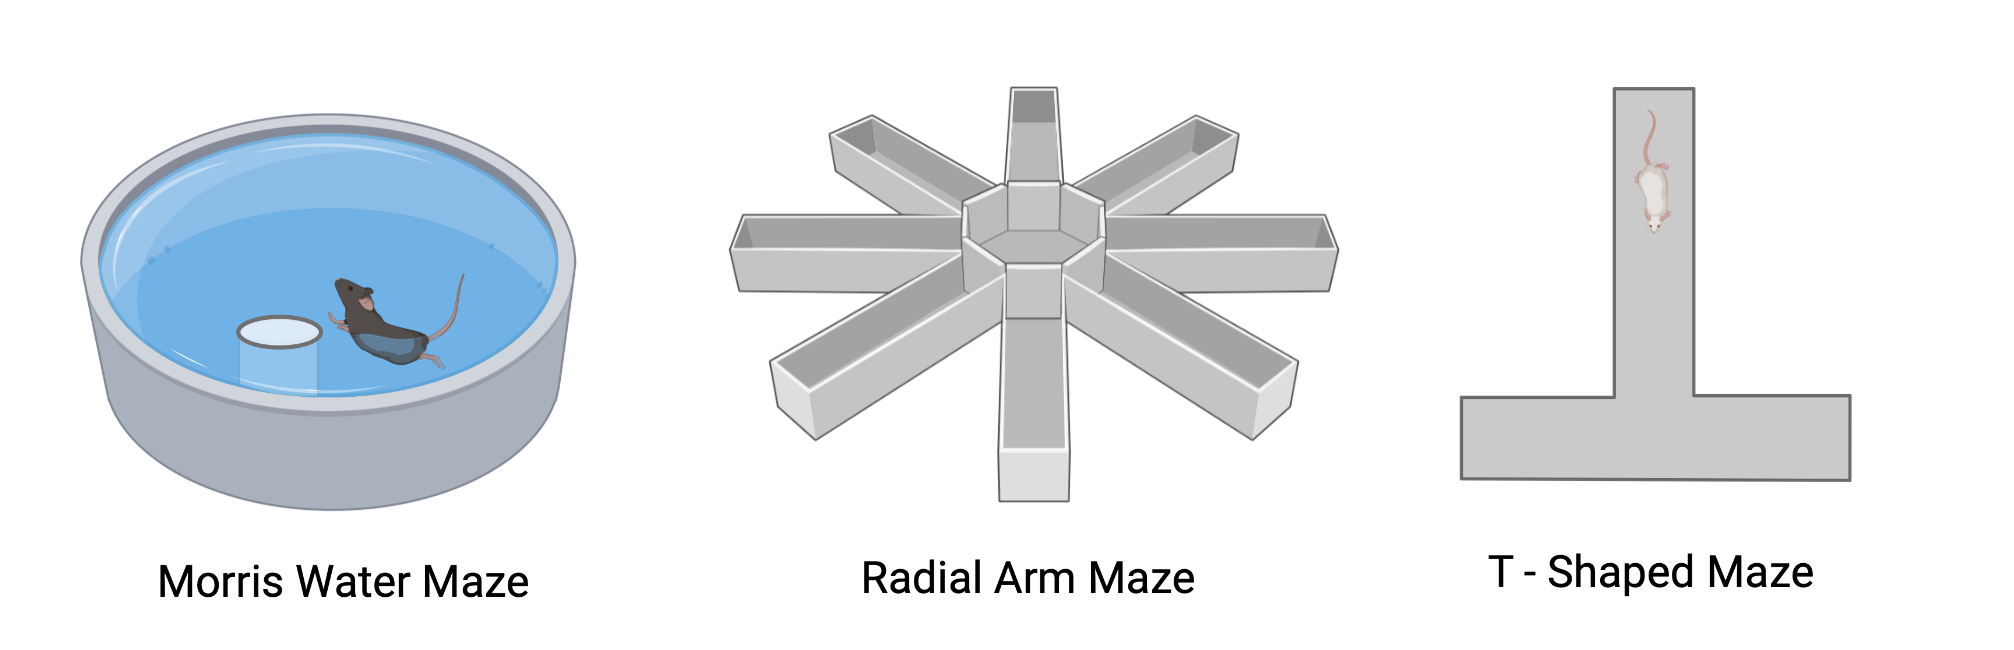
\includegraphics[scale=0.4]{images/previous_maze_designs.png}
    \caption{This figure shows previous designs of mazes used for investigating spatial memory of rodents.}
    \label{fig:previous_maze_designs}
\end{figure}

The important improvement that the Honeycomb Maze brings, is the ability to introduce many more choices for where the animal would like to move to: each time mouse is presented with a decision, it can choose between one of two possible choices.  Parameters such as angle of animal movement and distance to goal were also be correlated with the animals' navigation performance \cite{nature_honeycomb_maze_paper}. 

The Honeycomb Maze's makes is the ability to respond to the changing position of the animal poses a great advantage over static mazes such as the radial arm maze where the choices presented to the animal model are unchanging.
The Honeycomb Maze has been shown to be effective in investigating the cognitive maps of animal models \cite{nature_honeycomb_maze_paper} however, comes at the practical cost of building such a maze . This includes the financial cost of making the maze (approx. £100,000) in the laboratory as well as space required to do so, limiting movement choices for the animal.

The proposed solution is to use platform robots that are able to dynamically move around each-other to offer choices to the animal model. This design reduces the cost of building the maze to around £8,000. Further to this, the number of positions the animal model can navigate to is only limited by the size of the room not the relatively expensive cost of building more platforms from the previous design.

% \begin{tcolorbox}
\\

\paragraph{The aim of the dissertation} is to develop a tool for investigating behaviour of the animal models by implementing the Dynamic Honeycomb Maze Brief, providing a greater range of decisions the animal model can make.

% \end{tcolorbox}